\documentclass[11pt]{article}
\usepackage[margin=1in]{geometry}
\usepackage{amsmath,amssymb,booktabs,graphicx,caption,hyperref}
\newcommand{\rel}{\mathrm{relerr}}
\title{Global pCN under grid refinement: three observation arms}
\date{5 November 2026}
\begin{document}
\maketitle

\section{Summary of findings}
Nine runs (3 arms $\times$ grids $16^2,32^2,64^2$), each with 64 chains, $10^5$ iterations, adaptation to 25\% acceptance for the first $M=10^4$ iterations, state saved every 50 iterations. The parameter is the same 20-dimensional KLE vector on every grid, one fixed $\theta^*$.
\begin{itemize}
\item \textbf{With the relative-error likelihood the posterior and the sampler do not depend on the grid (arms 1 and 2).} The adapted step is $0.0513$ on all six runs, acceptance is $0.250$--$0.253$, MPSRF falls below $1.2$ after $21$--$22$k iterations, and the mean posterior sd of $\theta$ is $0.54$--$0.55$ everywhere. This holds whether the number of observations grows (arm 1: 128, 512, 2048) or is fixed (arm 2: 128 at the cell closest to each coarse checkerboard centre). The posteriors on the three grids agree to within the sampling noise of the runs (Section~\ref{sec:arms12}).
\item \textbf{With a fixed per-observation noise (arm 3) the posterior concentrates and pCN slows down in the way the information predicts.} The mean posterior sd falls from $0.547$ to $0.445$ to $0.324$, and the rms error of the posterior mean from $0.50$ to $0.45$ to $0.24$. The adapted step falls to $0.0260$ and $0.0132$, i.e.\ by $1.97\times$ and $3.89\times$, against $2.01\times$ and $4.03\times$ predicted from the growth of the Fisher-information trace ($4.05\times$, $16.2\times$).
\item \textbf{Arm 3 is not converged on the $64^2$ grid within $10^5$ iterations} (MPSRF $1.457$, max PSRF $1.403$ at the end); on $32^2$ it reaches $1.2$ only after $79$k iterations (versus $21$k on $16^2$). The $64^2$ posterior numbers of arm 3 (sd $0.324$, error $0.236$) are therefore provisional.
\item \textbf{The cost of converging grows much faster than the cost of an iteration.} Arm 3 needs about $4.9$\,s of CPU per chain to reach MPSRF $<1.2$ on $16^2$ and $80$\,s on $32^2$ ($16\times$), and more than $359$\,s on $64^2$ (a full $10^5$-iteration chain), at least $73\times$ the $16^2$ cost. Arms 1 and 2 are flat in iterations and grow only with the cost of the forward solve.
\item \textbf{The reference truth is now reproducible across machines.} The first version of this study produced different truths on two machines (Section~\ref{sec:kle}); the KLE basis is now fixed independently of the eigensolver.
\end{itemize}

\section{Setup}
\textbf{Problem.} Dirichlet permeameter on the unit square (pressure 1 left, 0 right, no flow top and bottom), cell-centred finite volume, squared-exponential kernel with correlation length $0.2$ and unit variance, $\log k=T\theta$, $\theta\sim N(0,I_{20})$. 20 modes hold $97.1\%$ of the variance.

\textbf{KLE (Section~\ref{sec:kle}).} The Nystr\"om problem is solved once on a $16\times16$-node Gauss--Legendre rule (full two-dimensional eigenproblem, no separability) and the 20 eigenfunctions are extended to the cell centres of each grid, so the three matrices $T_{16},T_{32},T_{64}$ sample the same eigenfunctions. The truth is $\theta^*=$ the first 20 standard normals of seed 2026. For the same $\theta^*$ the block-averaged $\log k$ differs between grids by $0.5$--$0.6\%$ and the block-averaged pressure by $0.04$--$0.05\%$, well below the $0.3\%$ data noise.

\textbf{Arms.}
\begin{center}\small
\begin{tabular}{@{}p{0.07\textwidth}p{0.36\textwidth}p{0.52\textwidth}@{}}\toprule
arm & observations & noise and likelihood\\ \midrule
1 check & checkerboard of the grid: 128 / 512 / 2048 & $\sigma_p=0.003\|p\|/\sqrt n$ ($2.09\cdot10^{-3}$); relative-error likelihood $\Phi=\|d-Op\|^2/(2\cdot0.003^2\|d\|^2)$\\
2 fixed & 128 on every grid: the grid cell closest to the centre of each $16\times16$ checkerboard cell (tie: lower-left of the central four) & as arm 1\\
3 abs & as arm 1 & fixed per-observation noise $\sigma_{\rm abs}=0.003\|p_{\rm obs,16}\|=0.0236$, Gaussian likelihood $\Phi=\sum r^2/(2\sigma_{\rm abs}^2)$\\ \bottomrule
\end{tabular}
\end{center}
With the relative-error likelihood the information per observation does not grow with the number of observations (numerator and $\|d\|^2$ both scale with $n$), which is why arm 3 was added. $\sigma_{\rm abs}$ makes the likelihood weight of arm 3 on $16^2$ equal to that of arms 1 and 2 ($1792$ against $1791$); the reasoning is in \texttt{docs/grid\_arms\_experiment.md}. The data of arm 3 carry about 11 times more noise than those of arms 1 and 2 (3.4\% against 0.3\% of the rms pressure).

\textbf{MPSRF and PSRF (group convention, \texttt{brho/mpsrf.py}), on the 20 coordinates of $\theta$.} The window starts at iteration $1000$, so the adaptation period is \emph{not} discarded, and it grows to the end of the run: at each curve point it holds the saved samples from the start to the current iteration, every 2nd sample, with a curve point every 15 saved samples. $W$ is the average within-chain covariance (divisor $n-1$), $B/n$ the covariance of the chain means (divisor $m-1$), $\mathrm{MPSRF}=\sqrt{(n-1)/n+(m+1)/m\,\lambda_{\max}(W^{-1}B/n)}$, and PSRF$_i=\sqrt{V_{ii}/W_{ii}}$ with $V=\frac{n-1}{n}W+\frac{m+1}{m}\frac Bn$; the maximum over components is reported. Not split-chain, no extra burn-in. ``Iterations to 1.2'' is the first curve point (ignoring the first 10) below $1.2$, interpolated linearly. $m=64$ chains.

\section{Results}
\begin{table}[h]\centering\footnotesize
\resizebox{\textwidth}{!}{\begin{tabular}{@{}lrrccccccccc@{}}\toprule
arm & grid & obs & step $s$ & median $\rel$ (at truth) & iter.\ to 1.2 (k) & MPSRF end & max PSRF end & mean sd $\theta$ & rms err.\ mean & KL to own $16^2$ & ESS proxy\\ \midrule
1 check & 16 & 128 & 0.0513 & 0.0115 (0.0033) & 22.1 & 1.045 & 1.038 & 0.543 & 0.349 & -- & 1410 \\
1 check & 32 & 512 & 0.0513 & 0.0116 (0.0032) & 21.7 & 1.053 & 1.046 & 0.546 & 0.340 & 0.10 & 1277 \\
1 check & 64 & 2048 & 0.0513 & 0.0115 (0.0030) & 22.4 & 1.051 & 1.046 & 0.544 & 0.338 & 0.13 & 1331 \\
\midrule
2 fixed & 16 & 128 & 0.0513 & 0.0115 (0.0033) & 22.1 & 1.045 & 1.038 & 0.543 & 0.349 & -- & 1410 \\
2 fixed & 32 & 128 & 0.0513 & 0.0115 (0.0033) & 21.7 & 1.053 & 1.048 & 0.549 & 0.351 & 0.04 & 1419 \\
2 fixed & 64 & 128 & 0.0513 & 0.0115 (0.0033) & 21.4 & 1.042 & 1.036 & 0.541 & 0.352 & 0.04 & 1400 \\
\midrule
3 abs & 16 & 128 & 0.0513 & 0.0362 (0.0375) & 21.1 & 1.046 & 1.040 & 0.547 & 0.501 & -- & 1364 \\
3 abs & 32 & 512 & 0.0260 & 0.0361 (0.0360) & 79.3 & 1.166 & 1.161 & 0.445 & 0.452 & 16.51 & 440 \\
3 abs & 64 & 2048 & 0.0132 & 0.0340 (0.0340) & none & 1.457 & 1.403 & 0.324 & 0.236 & 26.17 & 224 \\
\\ \bottomrule\end{tabular}}
\caption{All nine runs. Acceptance after adaptation is $0.250$--$0.256$ in all nine runs. Median relative error is taken after adaptation; ``at truth'' is the relative error of the noise realisation. KL is the Kullback--Leibler divergence of the Gaussian approximation (pooled post-$M$ mean and covariance) of the posterior from that of the same arm on $16^2$. ESS proxy: effective samples from the variance of the 64 chain means (median over coordinates, post-$M$ window).}
\end{table}

\begin{figure}[h]\centering
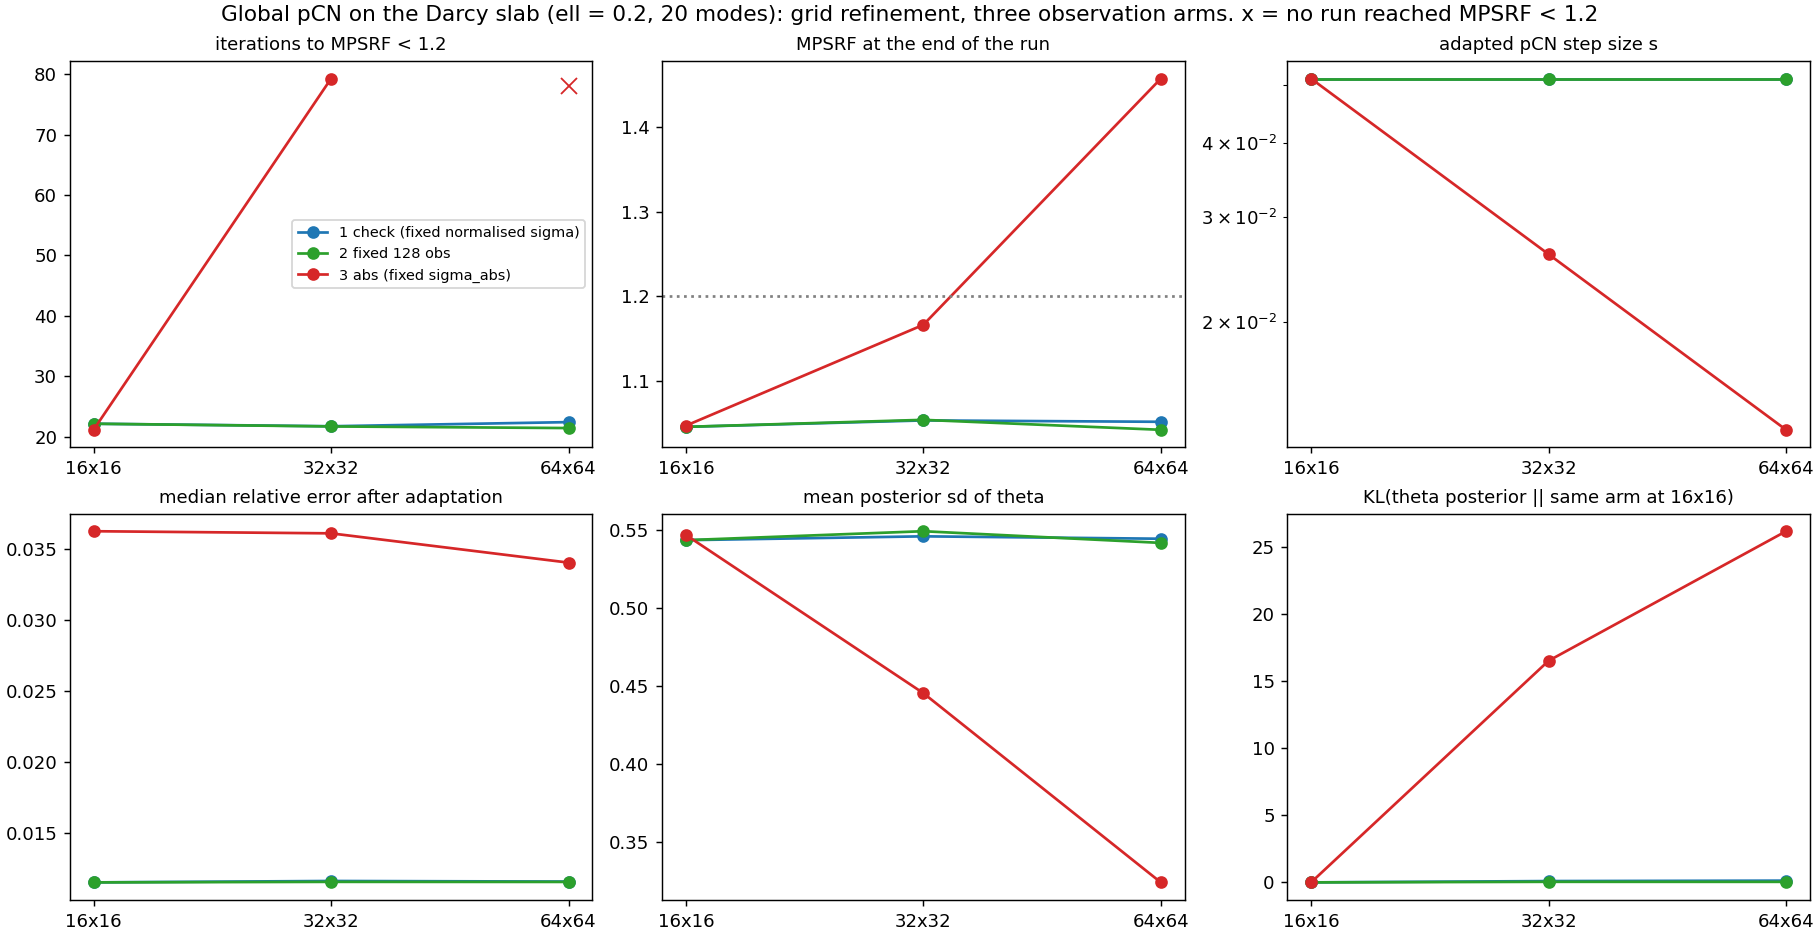
\includegraphics[width=\textwidth]{../compare/fig_scaling.png}
\caption{Grid scaling of the three arms. The cross marks the arm 3 run on $64^2$, which did not reach MPSRF $<1.2$. The posterior sd of $\theta$ and the KL divergence use pooled post-$M$ samples.}
\end{figure}

\subsection{Arms 1 and 2: grid independence}\label{sec:arms12}
Step size, acceptance, relative error, iterations to convergence and posterior spread are the same on all grids and in both arms, and the per-coordinate posterior sd curves of Figure~\ref{fig:sd} lie on top of each other. This is what the Fisher-information proxy ($\mathrm{tr}F$ within $1\%$ of the $16^2$ value in both arms) predicted. The KL divergences of the Gaussian fits from the $16^2$ fit are $0.04$--$0.13$. A rough noise floor for such a divergence between two independent fits of 20-dimensional Gaussians is $d(d+3)/(2N)$ with $N$ the effective number of samples; the chain-mean proxy gives $N\approx1.3$--$1.4\cdot10^3$ and a floor of $0.18$, so these differences are of the size of the sampling noise and I do not interpret them. The two arms agree with each other at every grid size. A caveat: both arms have a tempered likelihood (median $\Phi\approx7$ against about $0.6$ at the truth) and a posterior that is broad (mean sd $0.54$ against prior sd $1$), so this tests grid independence of the posterior and of pCN, not information gain.

\begin{figure}[h]\centering
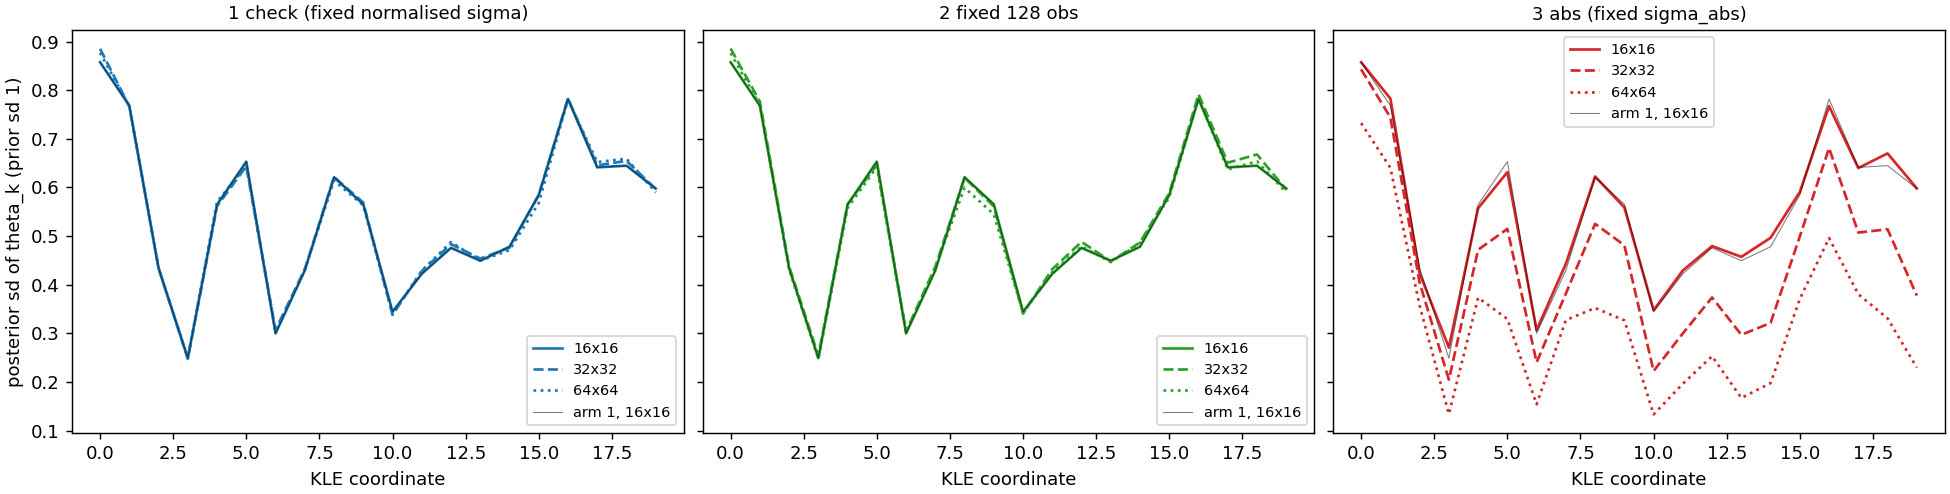
\includegraphics[width=\textwidth]{../compare/fig_theta_sd.png}
\caption{Posterior sd of each KLE coordinate on each grid. Arms 1 and 2 do not change with the grid; arm 3 shrinks in every coordinate.}\label{fig:sd}
\end{figure}

\subsection{Arm 3: concentration and slowdown}
At $16^2$ arm 3 has the same likelihood weight as arm 1 and its posterior is as wide ($0.547$ against $0.543$), but it is centred elsewhere (rms error of the mean $0.50$ against $0.35$; KL $9.8$) because its data carry a different, larger noise realisation. This is the intended design: arm 3 is compared with itself across grids. With refinement, the data constrain more directions (Fisher: $15,15,18$ directions above the prior's information; trace $4.05\times$ and $16.2\times$ the $16^2$ value), the posterior sd shrinks in every coordinate (to $0.37$--$0.85$ of its $16^2$ value on $64^2$; Figure~\ref{fig:sd}), the posterior-mean error falls ($0.50\to0.45\to0.24$) and the median relative error falls from $0.0362$ to $0.0340$, which equals the realised noise level at truth on each grid ($0.0375,0.0360,0.0340$). The median $\Phi$ ($73.6$, $291.0$, $1030.4$) sits at the values of the truth ($78.7$, $289.8$, $1031.7$), so the chains are in the region the noise model implies. The adapted step shrinks with the square root of the largest information eigenvalue, as predicted (Section~1).

\begin{figure}[h]\centering
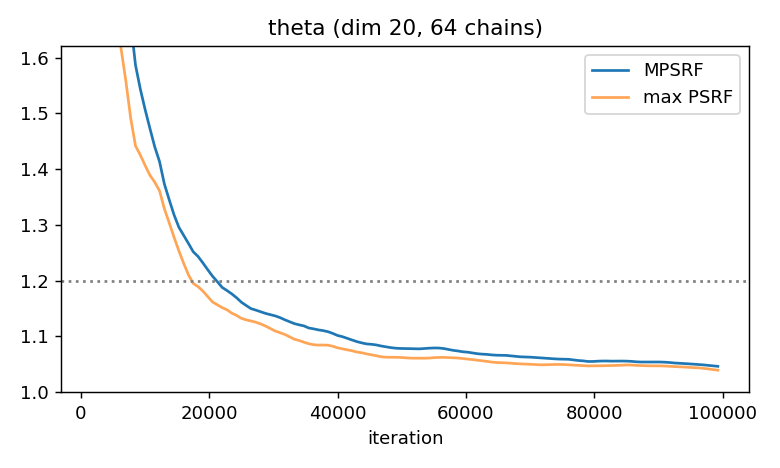
\includegraphics[width=0.49\textwidth]{../arm3_abs_n16/post/mpsrf_theta.png}\hfill
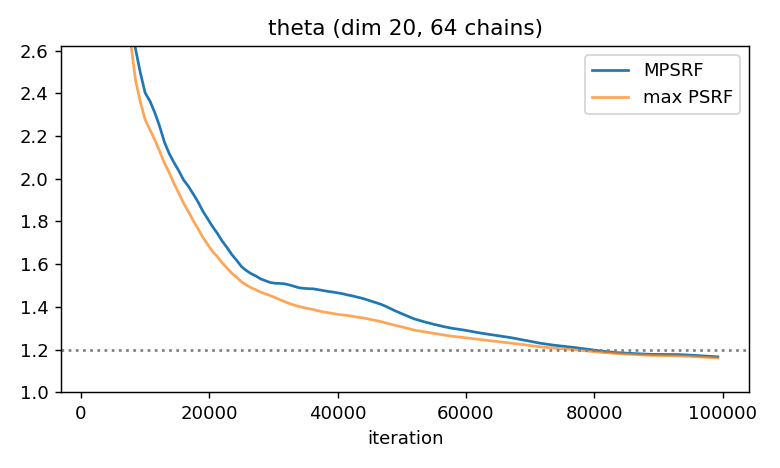
\includegraphics[width=0.49\textwidth]{../arm3_abs_n32/post/mpsrf_theta.png}\\[2mm]
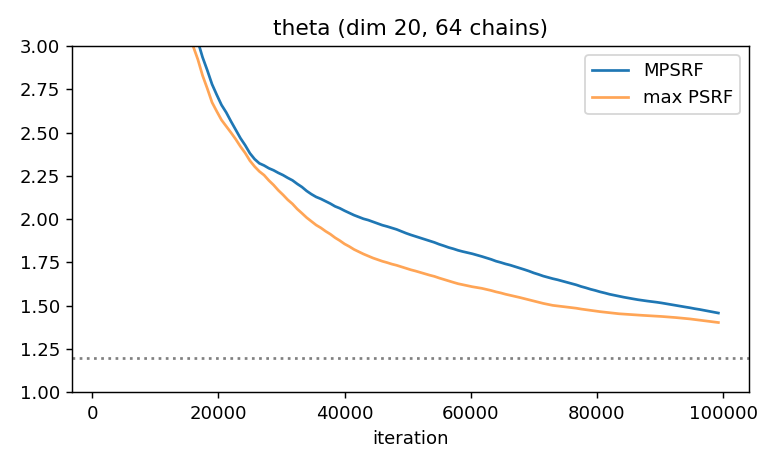
\includegraphics[width=0.49\textwidth]{../arm3_abs_n64/post/mpsrf_theta.png}
\caption{Arm 3 MPSRF and max PSRF of $\theta$ against iteration ($16^2$, $32^2$, $64^2$). The dotted line is $1.2$. Note the window includes the transient from iteration 1000 (Section~\ref{sec:caveats}).}
\end{figure}

\begin{figure}[h]\centering
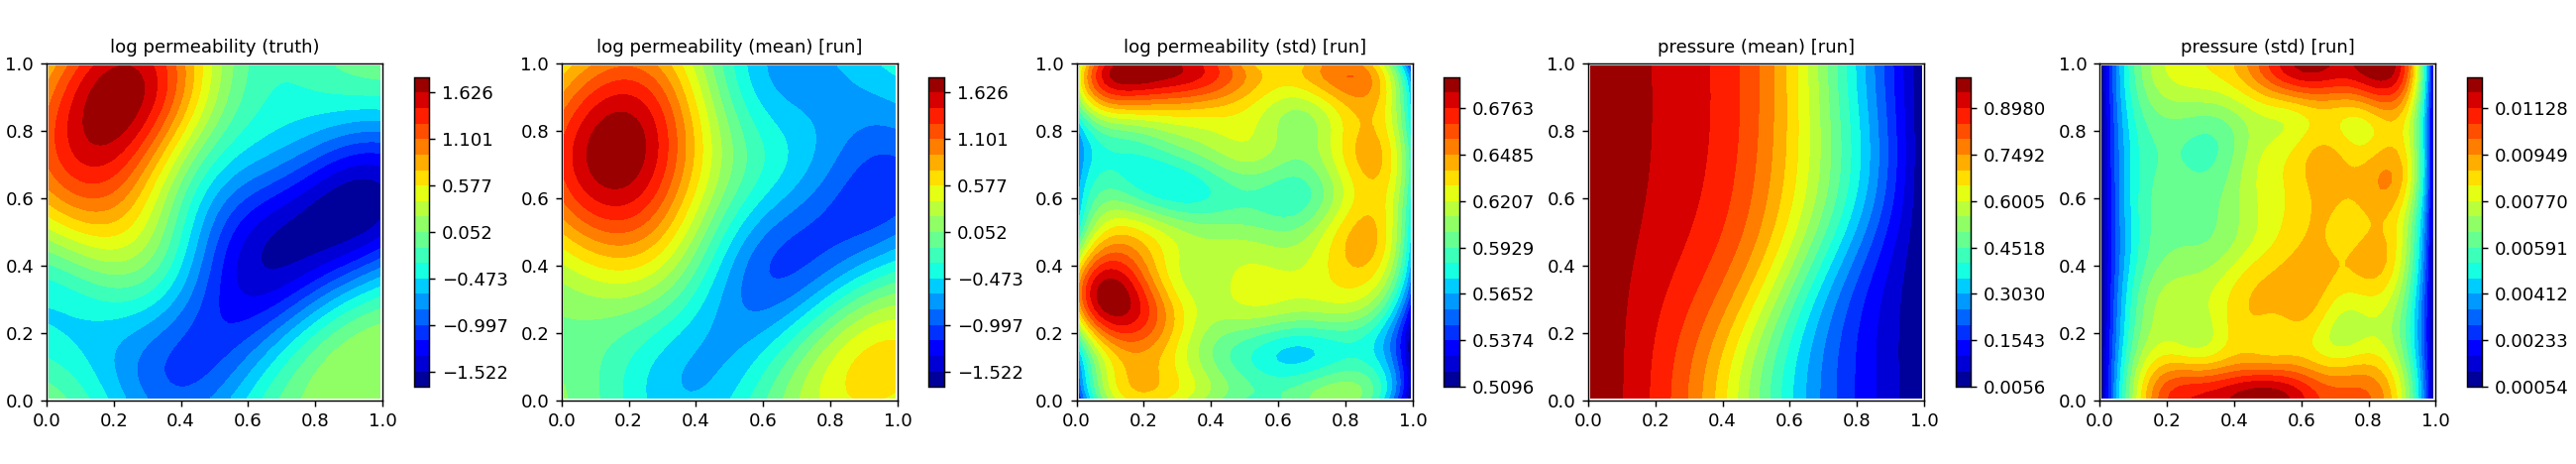
\includegraphics[width=\textwidth]{../arm1_check_n64/post/fields_run.png}\\
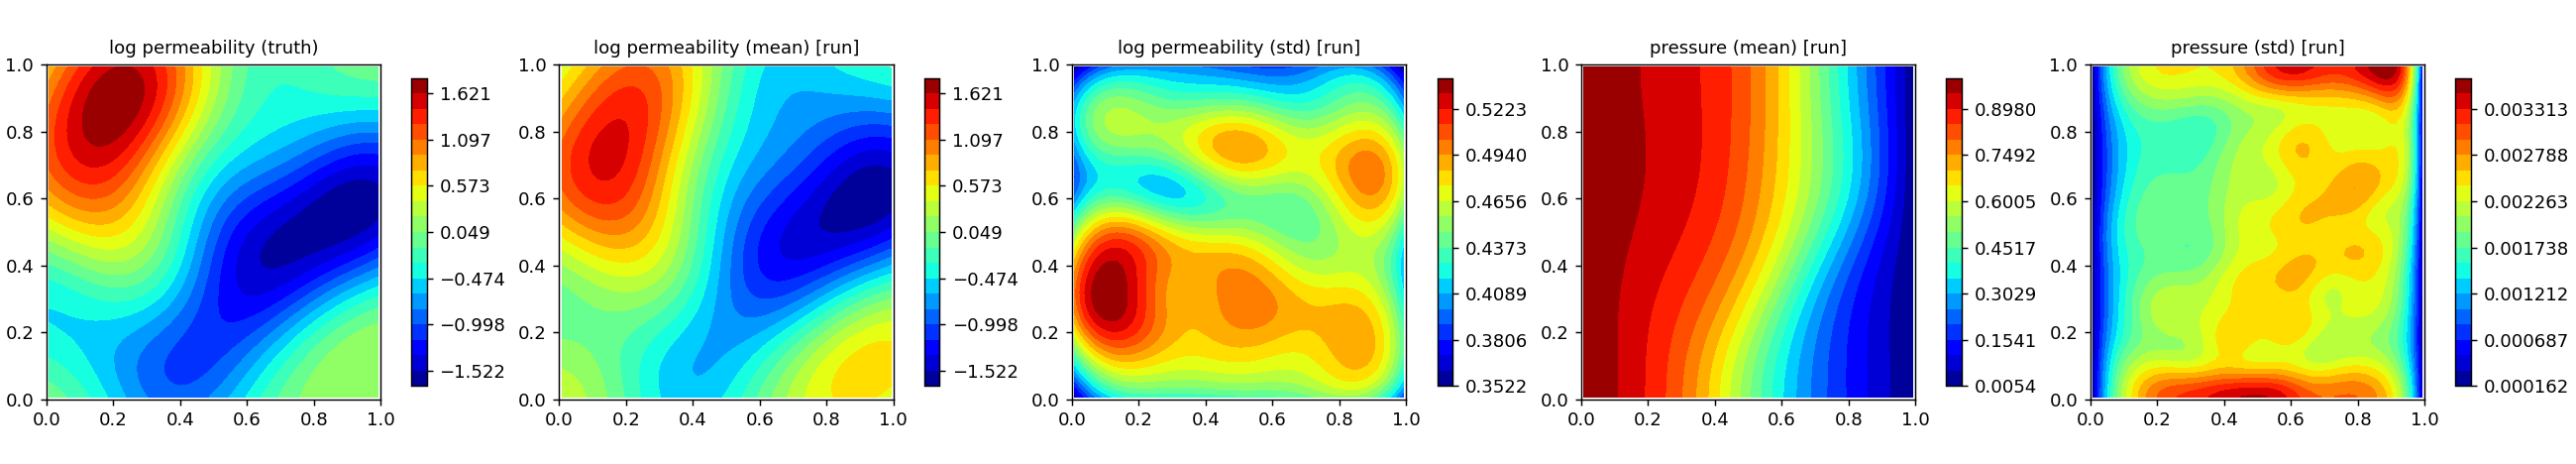
\includegraphics[width=\textwidth]{../arm3_abs_n64/post/fields_run.png}
\caption{Fields on the $64^2$ grid: arm 1 (top) and arm 3 (bottom): true $\log k$, posterior mean and sd of $\log k$, posterior mean and sd of the pressure (10\,000 pooled post-$M$ samples).}
\end{figure}

\section{The KLE and the reproducibility problem}\label{sec:kle}
In the first version of the study, built on the separable Nystr\"om KLE with eigenvector signs fixed by the largest entry, the same seed-2026 $\theta^*$ gave different truths on two machines ($\sigma_{\rm abs}=0.0167$ on the sandbox, $0.0240$ on the cluster), found by a unit test that compares $\sigma_{\rm abs}$ with a stored value. The seed fixes $\theta^*$, but not the basis it multiplies: an eigensolver returns eigenvectors only up to sign and, inside a degenerate eigenspace (the isotropic kernel on a square has the pairs $(i,j),(j,i)$), up to rotation, and the choice depends on the LAPACK build and library version. The final code uses \texttt{build\_kle(..., method="nystrom", basis="canonical")}, which fixes the basis of every degenerate group through the eigenspace projector (fixed smooth reference functions are projected onto the eigenspace and orthonormalised). $T$ then depends only on the kernel and the quadrature rule; the test now checks the value $\sigma_{\rm abs}=0.0236228$ on each machine and a second test randomly rotates the eigensolver's output inside tied groups.

\section{Caveats and what is not established}\label{sec:caveats}
\begin{itemize}
\item \textbf{Arm 3 on $64^2$ is not converged under this convention, but how much of that is the transient is not known from the repository.} The MPSRF window starts at iteration 1000 and grows to the end, so the transient stays in the window and only decays slowly (the relative error reaches the noise level within a few thousand iterations, but the stored outputs do not say how long the individual coordinates take to settle). The end value $1.457$ would be lower with a burn-in, and how much lower is unknown. \texttt{chains.npz} is not in the repository, so I did not recompute the curve with a burn-in. It is a quick computation on the cluster.
\item \textbf{The effective-sample proxy is rough.} It comes from the variance of 64 chain means and assumes each chain's mean is an unbiased estimate with variance $\mathrm{Var}/N_{\rm chain}$; for arm 3 on $64^2$ it gives about $220$ effective samples in total ($3.5$ per chain), so the Gaussian-fit quantities of that run (sd, KL to $16^2$: $26.2$) carry more sampling error than the others, in addition to the convergence question.
\item \textbf{One data set, one seed set.} All nine runs share $\theta^*$ and one noise stream per observation set. Differences of tens of percent in single-run iteration counts are not necessarily significant; the large effects (step size halving, MPSRF $1.05\to1.17\to1.46$, sd $0.55\to0.45\to0.32$) are well beyond that.
\item \textbf{KL values are of Gaussian approximations} of possibly non-Gaussian posteriors, to the arm's own $16^2$ fit, and say how much the posterior moved, not how far it is from the truth.
\end{itemize}

\section{Suggested next steps}
\begin{itemize}
\item Recompute the MPSRF of arm 3 on $32^2$ and $64^2$ with a burn-in (e.g.\ from iteration $5\cdot10^4$) from \texttt{chains.npz}, to separate transient from slow mixing.
\item If $64^2$ is genuinely unconverged, run it longer (about $2$--$4\cdot10^5$ iterations is about $0.7$--$1.4$\,h per chain at the observed $359$\,s per $10^5$ iterations on the cluster).
\item Optional arm 3b: $\sigma_{\rm abs}=0.0021$ (the literal $0.3\%$ noise), which should slow pCN much more; and a second seed for $\theta^*$ to check that the picture does not depend on one realisation.
\end{itemize}

\paragraph{Sources.} \raggedright In \path|runs/grid_arms_2026-11/|: \path|compare/table.json|, and for each run \path|post/post_summary.json| and \path|post/theta_stats.npz|. Fisher proxy: \path|tables/grid_arms/fisher_proxy.md|. Design and pilot: \path|docs/grid_arms_experiment.md|.
\end{document}
